\chapter{Introduction}
\lhead{\chaptername~\thechapter. \emph{Introduction}}
The growing interest of the general public in spherical cameras technologies, which were 
research-only exclusives once, has made them less expensive and more available. For example, omindirectional cameras by goPro have been extremely popular amongst sports men who publish them on social networks.

These devices have been employed in robotics since their first appearance to help navigate the robot in a real-world environment, and nowadays for autonomous driving. Furthermore, they can be exploited to deliver a virtual or augmented experience for augmented and virtual reality (AR/VR).

In this work, we designed a \textit{structure from motion} (SfM) pipeline for 
full spherical cameras. SfM is a well known topic in computer vision; it addresses the problem of 
recovering the structure of 3D environments from a sequence of images taken from different views.

SfM research (and computer vision in general) has targeted perspective cameras because these type of devices have always been more common. However, the increase of interest around these cameras has started a shift of interest towards employing them for research.

\section{Benefits of Full Spherical Cameras}
Because of the increased \textit{field of view} (FoV), panoramic cameras can capture a larger amount of data compared to traditional devices. For example, the two fisheye lenses in the Ricoh Theta allow users to utilize also rear correspondences between images and this may improve the quality of motion estimation.

Another advantage of full spherical cameras is that they do not require a calibration phase for intrinsic parameters estimation. Camera calibration is an essential requirement for most computer vision applications, which estimates several parameters such as focal length, image 
sensor size, pixel density, and lens distortion model. When dealing with full spherical cameras, we can assume the image is taken from a unitary sphere. Therefore, we can set the focal length to 1. Further details about the camera model and the parameters can be found in Chapter~\ref{ch:state_of_the_art}.

\section{SfM, VO, and SLAM}
SfM is a long studied topic in computer vision. Starting from an input of photographs taken by one or multiple cameras, SfM's main goal is to compute the cameras' poses and to reconstruct the 3D enviroment captured by those cameras.
%
Some of the first works are the paper by Longuet-Higgins\cite{longuet1981computer}, whose equations are fundamental in epipolar geometry, and the work by Tomasi et al.\cite{tomasi1992shape}, who used orthographic photographs to estimate the shape of a 3D object.
%
SfM is a general term, and it also includes \textit{visual odometry} (VO). This is the problem of recovering the motion of an agent equipped with a camera rig in a 3D environment. Typically, VO deals with an ordered set of images such as video sequences, and it uses them to compute the egomotion in real-time. Nister et al.\cite{nister2004visual} introduced the term \textit{visual odometry} for the first time.

Another field of robotic/computer vision research that is very close to VO is \textit{simultaneous localization and mapping} (SLAM). SLAM targets the problem of creating a map of the environment where a camera equipped agent navigates and simulatenously estimating its path. Scaramuzza\cite{scaramuzzaVisualOdometryI} pointed out that while VO is more focused on local motion estimation, SLAM's goal is to obtain a global consistent estimation of the agent movements.
%
In order to reduce error, SLAM keeps track of the visited path and can decide when the agent has come back to a previously visited location. This extra step in SLAM's pipeline is called \textit{loop closure} and provides an additional constraint used to reduce errors in both the agent's path and 
environment reconstruction. Durrant-White et al.\cite{durrant1996localization} firstly introduced the term SLAM.

%
% Francesco
%
 
\section{Densification: from Sparse to Dense Point Cloud}
\textbf{NOTA: perche' questo discorso e' solo per VO e non SfM SLAM?}
A sparse point cloud is the product of most VO pipelines; some key points are tracked in each photograph and are then used by the motion estimation algorithm. These key points are triangulated and their corresponding world points are available during egomotion estimation.
%
A set of triangulated key points is a sparse point cloud around the camera's path. This set provides a first approximation of the environment reconstruction.
Densification algorithms increase the number of matched points in two consecutive frames, this allows us to triangulate these points too. The result is a dense cloud of points around the camera's path that provides additional information about the surroundings' geometry.

\section{Omnidirectional and Full Spherical Cameras}
\label{sec:cameraclassification}
Omnidirectional cameras are characterized by wide field of view. Indeed, many of this kind of devices can take pictures with a 180\degree view angle or even wider.

There are several ways to obtain panoramic images, they include:
\begin{itemize}
	\item perspective cameras and image stitching;
	\item catadioptric cameras;
	\item dioptric cameras;
	\item hybrid approaches.
\end{itemize}

\textbf{NOTA: citare software come Hugin: http://hugin.sourceforge.net/}
\textbf{NOTA: citare spheron VR: https://www.spheron.com/home.html}

Perspective cameras can take panoramic pictures with the aid of software stitching. As the first step, we take several photographs with many cameras or by simply moving the same camera in order to cover most of a scene. Then, a stitching software merges all images into a single one. To use a traditional camera and a stitching software is the cheapest way to obtain panoramic images because it does not need any kind of specialized hardware. However, this process is cumbersome (i.e., a lot of manual work for the user), and most importantly video sequences cannot be recorded. Note that some smart-phones provide built-in camera 360\degree acquisition modes, but the final quality may be not satisfactory due to alignment artifacts.

Catadioptric cameras are obtained with a perspective camera and a mirror mounted in front of it. The camera take a picture of the mirror that reflects the surrounding. The mirror of a catadioptric system may have several shapes. The most common one is the hyperbolic profile that creates a single center of 
projection for every ray coming to the mirror.

\textbf{NOTA: fa l'esempio della goPro}
A traditional camera can also be adapted to work as a panoramic one by adding a fisheye lens capable of refracting lights from wide angle towards the image sensor. These setups are called dioptric cameras.

Apart of perspective cameras coupled with stitching software, none of the previous approaches can take full spherical panoramic photographs. Moreover, full spherical videos cannot be shot with perspective cameras either.

The last approach, an hybrid one, exploits several sensors using fisheye lenses and software stitching to capture full spherical panoramic images in a single shot. This enables full spherical video capturing as well. The camera (that is composed of several image sensors) take multiple overlapping pictures simultaneously. Then, an on camera stitching software composes the data in a single image.

In all our experiments we used the Ricoh Theta S camera that is a hybrid full spherical camera 
composed of two fisheye lenses with a FOV greater than 180\degree; see Figure~\ref{fig:ricoh_theta}.

\begin{figure}
\centering
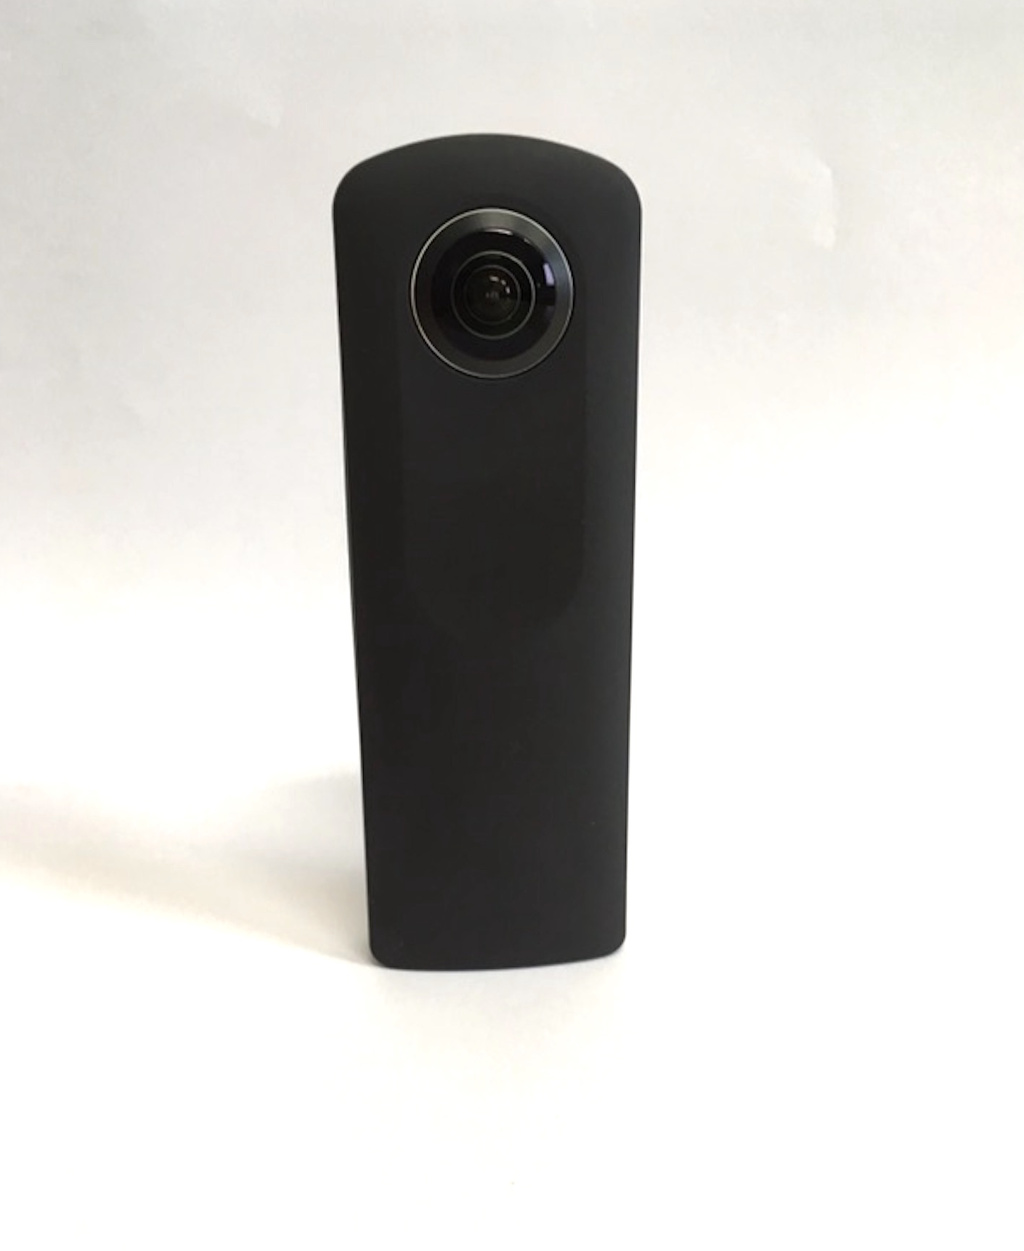
\includegraphics[width=0.7\textwidth]{img/theta1}
\label{fig:ricoh_theta}
\caption{The Ricoh Theta S 360\degree camera.}
\end{figure}
